\chapter{Sensitivity Analysis}
\label{ch:SensitivityAnalysis}
In this chapter, the sensitivity of the trade-off is analysed, in order to validate the trade-off and to ensure that the correct concept is chosen.
The trade-off first chooses criteria and then gives each criterion a weight, after which each concept is graded on each criterion and a final grade per concept is obtained.
This process evaluates the sensitivity of the criteria and their weights.
%In this chapter, the sensitivity of the criteria and their weights is analysed in depth. 
It is assumed that the grading per criterion for the designs cannot be changed; otherwise, the entire trade-off would be redundant.
To evaluate the trade-off, first, a criteria analysis is performed, followed by a weight analysis.

\section{Criteria Analysis}
\label{sec:WeightChangeSensitivity}
To see how much the winner of the trade-off depends on the chosen criteria, the trade-off is performed six times, each time removing a different criterion entirely.
If a new winner arises every time a different criterion is removed, the trade-off is too sensitive and needs to be changed.
The results from these trade-offs are given in \Cref{tab:critremove}.

\begin{table}[ht]
    \centering
    \caption{Trade-off winners with five out of six criteria active}
    \label{tab:critremove}
    \begin{tabular}{l|m{1cm}m{1.8cm}m{2cm}m{1.8cm}m{1cm}m{1.7cm}}
        \toprule
        \textbf{Criterion removed}&  TRL &  Transition efficiency &  Structural complexity &  Energy consumption &  Safety & Noise emissions \\ \midrule
        \textbf{Winner}&  \ref{C2.1} &  \ref{C1.5} &  \ref{C2.1} &  \ref{C2.1} &  \ref{C2.1} & \ref{C2.1} \\ \bottomrule
    \end{tabular}
\end{table}

\section{Weight Analysis}
\label{sec:GradingChandeSensitivity}
Now that all the criteria have been validated, it is necessary to look at the weights of the criteria and analyse if changing these weights will change the outcome of the trade-off.
This is realised by changing the weights such that a weight can become 0.05 higher or 0.05 lower.
The value of 0.05 is chosen since most criteria are 0.05 from each other.
Evidently, the total of the weights still needs to add up, so if the weight of one criterion increases by 0.05, the weight of another criterion decreases by 0.05, or one weight decreases by 0.02 and another with by 0.03, which allows for around 100.000 different combinations.
The only rules for the weights are that the end weights should stay within ±0.05 of the original weight, and the sum of all the weights remains 1.00.
The weight ranges can be seen in \Cref{tab:CritWeight}.

\begin{table}[ht]
    \centering
    \caption{Criteria weight ranges}
    \label{tab:CritWeight}
    \begin{tabular}{l|m{1.5cm}m{1.8cm}m{2cm}m{1.8cm}m{1.5cm}m{1.7cm}}
        \toprule
         &  TRL&  Transition efficiency&  Structural complexity&  Energy consumption&  Safety& Noise emissions\\ \midrule
         \textbf{Weight}&  0.10&  0.30&  0.15&  0.20&  0.10& 0.15\\
         \textbf{Weight range}&  0.05-0.15&  0.25-0.35&  0.10-0.20&  0.15-0.25&  0.05-0.15& 0.10-0.20\\ \bottomrule
    \end{tabular}
\end{table}

The trade-off is performed for each combination of weights, so the final grades can be calculated.
The distribution of the final grades per concept can be seen in the kernel density plot \Cref{fig:KDEPlot_weightChange}.
From all the performed trade-offs, the rotating wing design wins 98\% of the time, the other 2\% was won by the Winged Rotorcraft.

\begin{figure}[ht]
    \centering
    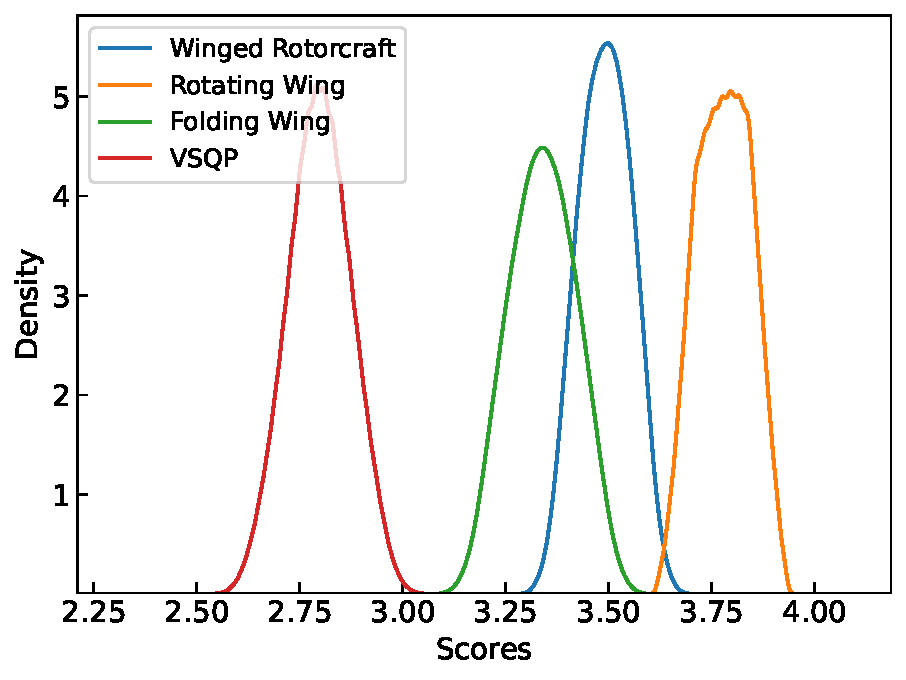
\includegraphics[width=0.7\linewidth]{figures/Sensitivity/sensitivity.pdf}
    \caption{Kernel density plot of the final score distribution per concept}
    \label{fig:KDEPlot_weightChange}
\end{figure}

\section{Trade-Off Conclusion}
\label{sec:TradeOffConlusion}
To conclude the sensitivity analysis, the results of both types of analysis are discussed in the following.
The criterion analysis can be considered inconclusive if, for all dropouts, a new winner emerges.
As it can be seen from \Cref{tab:critremove} it is not the case.
It can be deduced that the Rotating Wing design overperforms by losing the trade-off only once, hence the analysis can be considered successful.

Continuing with the weight analysis,
the winner and the trade-off can be considered stable
if the initial winner can surpass the other contestants in at least 70 \% of the iteration.
As stated in the previous section, the initial winner wins 98\%,
which can be considered acceptable with high confidence.
Furthermore, \Cref{fig:KDEPlot_weightChange}
shows that the only concept that can overperform the Rotating wing concept is the Winged Rotorcraft.

Therefore, the final conclusion can be drawn from the two analyses; the trade-off can be firmly stable, whilst the Rotating Wing concept obtained a strong first place among the other designs.
